 \documentclass{report}
 
\usepackage[utf8]{inputenc} 
\usepackage[T1]{fontenc}      
\usepackage[top=3.5cm, bottom=3cm, left=3.0cm, right=4.0cm]{geometry}
\usepackage{graphicx}
\graphicspath{{figures/}{../figures}}

\begin{document}

\chapter*{Association en cascade, AO en régime linéaire et saturé, courbes intensité-potentiel}

\newpage

\section*{Exercice 1}

Le cadre en pointillé représente un quadripôle tel que : $u_{s}=Gu_{e}$.

\begin{itemize}

\item[•] On suppose d'abord que $R_{s}=0$ et $R_{e}=\infty$. Trouvez  une équation différentielle en $i(t)$. Quelle est la condition sur $G$ pour voir apparaître des oscillations ? Donnez alors la valeur $f_0$ des oscillations.

\item[•] Comment cette condition change lorsque $R_{s}\neq 0$ et $R_{e}\neq\infty$?

\end{itemize}

\begin{figure}[!h]
\centering
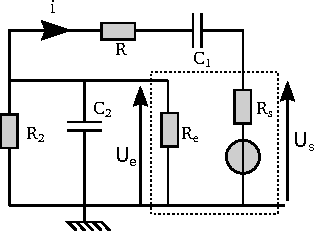
\includegraphics[width=0.5\linewidth]{circuit_5.pdf}
\end{figure}

\newpage

\section*{Exercice 2}

On considère le montage suivant.

\begin{figure}[!h]
\centering
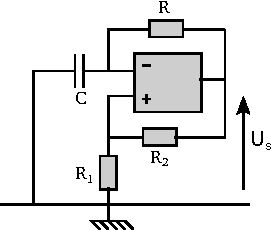
\includegraphics[width=0.45\linewidth]{circuit_3.pdf}
\end{figure}

\subsubsection{Amplificateur idéal}

On suppose l'AO idéal : rappeler ses caractéristiques. Dans la suit, on notera $\tau_1=RC$.

\begin{itemize}
	\item[$\clubsuit$] Comment se comporte t-il dans cette situation ? Pourquoi ?
	\item[$\clubsuit$] Déterminez l'évolution temporelle de  $U_{-}(t)$ et $U_{s}(t)$. 
\end{itemize}

\subsubsection{Amplificateur réel}

On considère désormais que l'amplificateur est réel, c'est-à-dire que les tensions $u_+$, $u_-$ et $u_s$ vérifient la relation suivante : 
	\begin{equation}
		\tau_0\frac{du_s}{dt} +u_s = \mu_0(u_+-u_-)
	\end{equation}
	avec $\mu_0=10^5$ et $\frac{\mu_0}{2\pi\tau}=$1MHz.
\begin{itemize}
	\item[$\clubsuit$] Déterminez une équation différentielle sur $u_s(t)$. Commenter les solutions. 
	\item[$\clubsuit$] Si l'on considère nulles la tension de sortie ($u_s(t=0)=0$) et la tension aux bornes du condensateur  ($u_-(t=0)=0$), pourquoi se retrouve t-on rapidement dans la situation précédente, cad avec des oscillations sur $u_s(t)$ ?
\end{itemize}


\newpage

\section*{Exercice 3}

On considère le circuit ci-dessous :

\begin{figure}[!h]
\centering
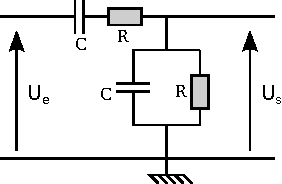
\includegraphics[width=0.5\linewidth]{circuit_1.pdf}
\end{figure}

\begin{itemize}
	\item[•] Après avoir précisé le comportement du circuit en basse et haute fréquence, déterminez la fonction de transfert de ce filtre sous la forme canonique. Quelle est l'allure de son diagramme de Bode ?
	\item[•] On réalise ce désormais le montage avec l'AO. Pour quelles valeurs de $R_1$ et $R_2$ voit-on apparaître des oscillations sur $U_{e}$?
\begin{figure}[!h]
\centering
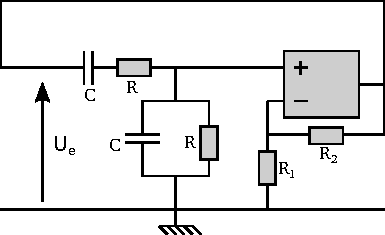
\includegraphics[width=0.6\linewidth]{circuit_4.pdf}
\end{figure}

	\item[•] Pourquoi parle t-on de régime quasi-sinusoïdal ? Décrire l'évolution du signal si les oscillations apparaissent à partir du bruit de fond électronique.
\end{itemize}


\newpage

\section*{Exercice 4}

On considère le circuit ci-dessous :

\begin{figure}[!h]
\centering
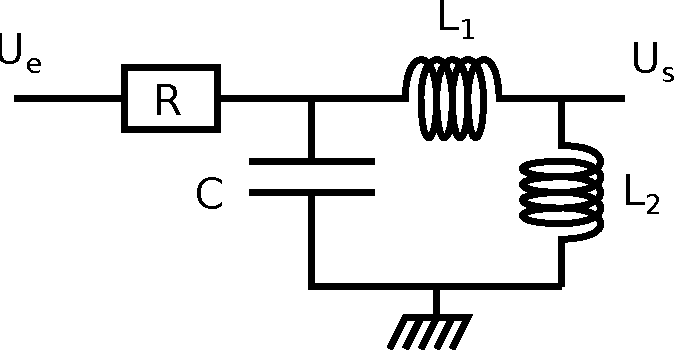
\includegraphics[width=0.4\linewidth]{resonnateur.pdf}
\end{figure}

\begin{itemize}
	\item[•]  Après avoir précisé le comportement du circuit en basse et haute fréquence, déterminez la fonction de transfert de ce filtre sous la forme canonique.
	\item[•] A quelle condition a t-on des oscillations sur le circuit avec le montage ci-dessous ?
	
	\begin{figure}[!h]
\centering
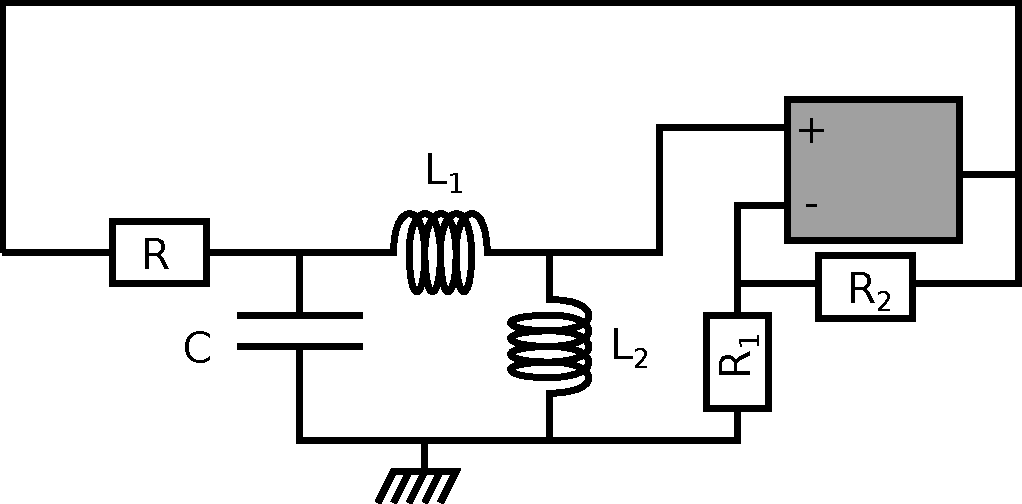
\includegraphics[width=0.4\linewidth]{resonnateur2.pdf}
\end{figure}

	\item[•] Pour éviter d'atteindre la saturation de l'AO en régime quasi-sinusoïdal, on suppose que $R_1$ est une thermorésistance, cad dont la résistance augmente proportionnellement avec la température. Expliquez comment cela permet d'éviter la saturation de l'AO.

\end{itemize}




\subsection*{Exercice supplémentaire}
Est-il possible d'avoir des oscillations sur un tel circuit si H est un passe-bas d'ordre 2 ? A quelles conditions ? 
Même questions pour un passe haut d'ordre 2.
\begin{figure}[!h]
\centering
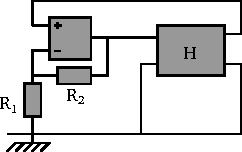
\includegraphics[width=0.3\linewidth]{circuit_9.pdf}
\end{figure}

\newpage

\section*{Remplissage d'un réservoir d'hélium}
\subsection*{Première version}
On considère ici un système de remplissage d'un réservoir d'hélium. Par évaporation, de l'hélium s'échappe constamment du réservoir. Pour des raisons pratiques, on souhaite maintenir le niveau d'He à un niveau minimum $h_{min}$.

Pour cela, une vanne (V) introduit de l'hélium dès que la tension à ses bornes est positive. Pour mesurer le niveau d'He, un transducteur (T) fournit une tension $e$ proportionnelle à la hauteur d'He : $e= \alpha h$. (P) est un potentiomètre dont la résistance varie de $0$ à $800\Omega$.

\textit{Données : $R_{1} = 100$k$\Omega$, $R_{2}=R_{3}=200\Omega$, $\alpha = 5V/m$. L'AO est supposé idéal et sa tension de saturation est $V_{sat+}=10V$ et $V_{sat-}=0V.$}

\begin{figure}[!h]
\centering
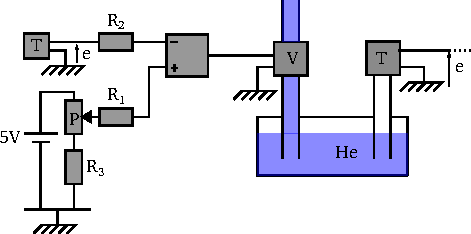
\includegraphics[width=0.8\linewidth]{circuit_10.pdf}
\end{figure}

Comment fonctionne ce montage ? Donnez la hauteur minimale $h_{min}$ et maximale $h_{max}$. Quel est le défaut de ce système ?

\subsection*{Seconde version}
On introduit une rétroaction sur l'AO avec une résistance.

\begin{figure}[!h]
\centering
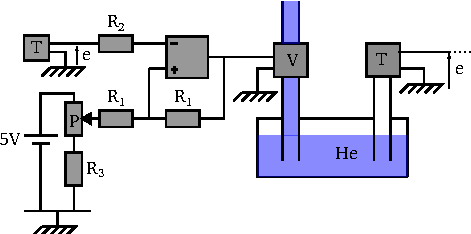
\includegraphics[width=0.8\linewidth]{circuit_11.pdf}
\end{figure}

Comment fonctionne ce nouveau montage ? Quel est son intérêt ? Donnez la hauteur minimale $h_{min}$ et maximale $h_{max}$.

\newpage

\section*{Électrolyse du sulfate de cobalt}

La solution a électrolyser renferme de l'acide sulfurique (considéré comme un diacide fort), du sulfate de cobalt et du sulfate de cuivre (qui seront supposé entièrement dissociés). 

Avant de réaliser l'électrolyse proprement dite, le cuivre est éliminé par cémentation du cuivre par le fer (opération durant laquelle la solution est chauffée au contact de la poudre de fer sous agitation et contrôle du pH).

L'électrolyse est réalisée dans une cuve en ciment revêtue de PVC, en maintenant une température constante entre une anode (A) en graphite et une cathode (C) en aluminium. Le pH de l'électrolyte est stabilisé à une valeur de 3.

La solution initiale à électrolyser ne referme plus d'ions Fe$^{2+}$  et contient CoSO$_4$, 7H$_2$O à la concentration massique de 50g.L$^{-1}$. 

\textit{Pour simplifier, les calculs de potentiels seront effectués dans les conditions standards à 25$^\circ$C, excepté pour les concentrations en $H_3O+$ et Co$^{2+}$ qui seront celles de l'électrolyse (ph=3).}

\begin{itemize}
	\item[•] Quelle est l'équation-bilan traduisant la cémentation ? En utilisant les données, justifier avec un tracé de courbes intensité-potentiel la possibilité d'éliminer seulement les ions Cu$^{2+}$. 
	\item[•] Quelles sont les réactions les plus favorisées thermodynamiquement à l'anode et à la cathode ? Quelle tension minimum faut-il appliquer pour obtenir une électrolyse ? 
	\item[•] Représenter schématiquement, en tenant compte des surtensions, l'allure des courbes intensité-potentiel correspondantes. Quelle réaction est alors privilégiée ?
	\item[•] Ecrire l'équation-bilan de l'électrolyse. Celle-ci est-elle sous contrôle thermodynamique ou cinétique ?
\end{itemize}
\textit{La chute ohmique relative aux électrodes et à l'électrolyte s'élève à 1,1V.}
\begin{itemize}
	\item[•] Déterminer la tension minimale de fonctionnement de la cuve d'électrolyse. 
\end{itemize}
\textit{L'électrolyse est réalisée sous une tension de 3,5V avec une intensité de 10kA, et une densité de courant de 400A.m$^2$.}
\begin{itemize}
	\item[•] Calculer la masse théorique de Co métal obtenue à l'issue d'un jour d'électrolyse. 
\end{itemize}
\textit{La masse de Co réellement obtenue sur une journée est de 256kg.}
\begin{itemize}
	\item[•] Définir puis calculer le rendement faradique. Expliquer pourquoi ce rendement ne peut atteindre 100$\%$.
	\item[•] Déterminer la consommation massique d'énergie en kJ.kg$^{-1}$ (énergie nécessaire à la production d'un kg de Co).
\end{itemize}

\textit{Données}

\vspace{0,2cm}
\begin{tabular}{|c|c|c|c|c|c|}
\hline
Couple & Co$^{2+}$/Co &  H$_3$O$^{+}$/H$_2$ & O$_2$H$_2$O & Cu$^{2+}$/Cu & Fe$^{2+}$/Fe\\
\hline
E$^\circ$(V) & -0,29 & 0,00 & 1,23 & 0,34 & -0,44\\
\hline
\end{tabular}

Surtensions aux électrodes : 

$\eta_C$(Co), sur Fe : -0,15V ;
$\eta_C$(H$_2$), sur Al : -0,4V ;
$\eta_C$(Co), sur Al : -0,1V ;
$\eta_A$(O$_2$), sur graphite : 0,7V ;

Constantes : 

$RTln10/F=0,060$V (à 298K), constante de Faraday : 96500C.mol$^{-1}$.

Masse molaire (en g.mol$^{-1}$) : M(H)=1,0 ; M(O)=16,0 ; M(S)=32,1 ; M(Co) = 58,9. 

Numéros atomiques : Co : 27, N : 7 et H : 1




\end{document}
